\documentclass[tikz,border=5pt]{standalone}
\usepackage{pgfplots}
\pgfplotsset{compat=1.18}

\definecolor{trosA}{HTML}{365FB3}
\definecolor{trosB}{HTML}{7C3AED}
\definecolor{punt}{HTML}{C2415D}
\definecolor{guia}{HTML}{6B7280}

\begin{document}
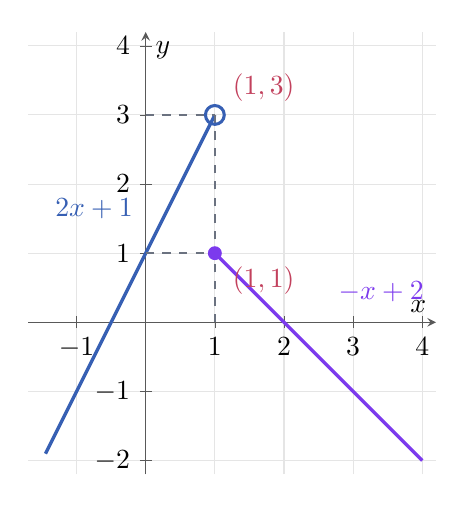
\begin{tikzpicture}
  \begin{axis}[
    width=10.8cm,
    height=7.2cm,
    axis lines=middle,
    xmin=-1.7,
    xmax=4.2,
    ymin=-2.2,
    ymax=4.2,
    axis equal image,
    xlabel={$x$},
    ylabel={$y$},
    xtick={-1,1,2,3,4},
    ytick={-2,-1,1,2,3,4},
    axis line style={black!65},
    tick style={black!65},
    grid=major,
    grid style={black!10},
    clip=false,
  ]
    \addplot[trosA, very thick, domain=-1.45:1, samples=100]
      {2*x+1};
    \addplot[trosB, very thick, domain=1:4, samples=100]
      {-x+2};

    \addplot[guia, dashed, thick] coordinates {(1,0) (1,3)};
    \addplot[guia, dashed, thick] coordinates {(0,3) (1,3)};
    \addplot[guia, dashed, thick] coordinates {(0,1) (1,1)};
    \addplot[
      only marks,
      mark=o,
      mark size=3.4pt,
      trosA,
      mark options={draw=trosA, fill=white, line width=1.1pt}
    ] coordinates {(1,3)};
    \addplot[only marks, mark=*, mark size=2.3pt, trosB]
      coordinates {(1,1)};

    \node[anchor=south west, text=trosA]
      at (axis cs:-1.45,1.35) {$2x+1$};
    \node[anchor=south west, text=trosB]
      at (axis cs:2.65,0.15) {$-x+2$};
    \node[anchor=south west, text=punt]
      at (axis cs:1.12,3.06) {$(1,3)$};
    \node[anchor=north west, text=punt]
      at (axis cs:1.12,0.94) {$(1,1)$};
  \end{axis}
\end{tikzpicture}
\end{document}
